\subsection{ระบบที่ใช้ช่วยในการพัฒนาหุ่นยนต์}
Robot Middleware เป็นกรอบการทำงาน (framework) ที่มีความยืดหยุ่นสำหรับการพัฒนาซอฟแวร์ที่ซับซ้อนในการควบคุมของหุ่นยนต์
ตัว Robot Middleware ถูกออกแบบมาให้ใช้ในการจัดการระบบที่มีความยุ่งยาก โดยมีเครื่องมือที่ช่วยติดต่อสื่อสารระหว่างอุปกรณ์ต่างๆของหุ่นยนต์ 
Robot Middleware ส่วนใหญ่จะใช้การติดต่อสื่อสารผ่านระบบเครือข่ายเน็ตเวิร์ค ทำให้การสื่อสารในระบบพื้นฐานเป็นอิสระต่อกัน 
และสามารถติดต่อสื่อสารกันกับอุปกรณ์ที่อยู่ภายนอกผ่านเครือข่ายเดียวกันได้

ปัจจุบันมี Robot Middleware ที่ถูกพัฒนาขึ้นมาให้ใช้อยู่หลายตัวเช่น

\subsubsection*{Player Project}
\begin{figure}[!ht]
    \centering
    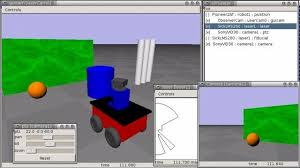
\includegraphics[width=0.45\textwidth]{chapter2/images/mdw_playerproject.jpeg}
    \caption{player project middleware}
    \label{fig:mdw_playerproject}
\end{figure}
เป็นโปรเจคที่ใช้ในการสร้างซอฟแวร์เพื่อการศึกษาวิจัยที่มีความเกี่ยวข้องกับหุ่นยนต์และระบบเซนเซอร์
ภายในประกอบไปด้วยระบบตัวกลาง และระบบจำลองการทำงานของหุ่นยนต์

\subsubsection*{YARP}
\begin{figure}[!ht]
    \centering
    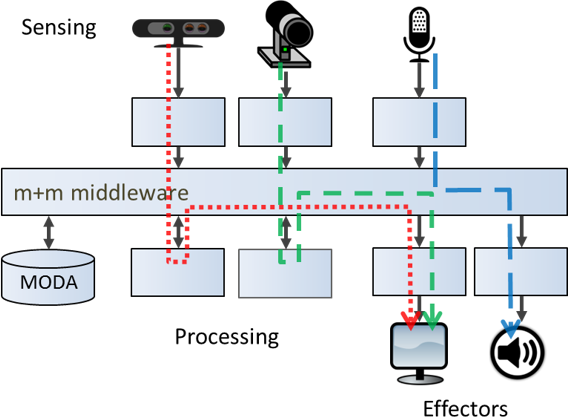
\includegraphics[width=0.45\textwidth]{chapter2/images/mdw_yarp.png}
    \caption{yarp middleware}
    \label{fig:mdw_yarp}
\end{figure}
เป็น open source ที่เขียนด้วยภาษา C++ ในการเชื่อมต่อกับเซนเซอร์ หน่วยประมวลผล และตัวขับเคลื่อนของหุ่นยนต์

\clearpage
\subsubsection*{URBI}
\begin{figure}[!ht]
    \centering
    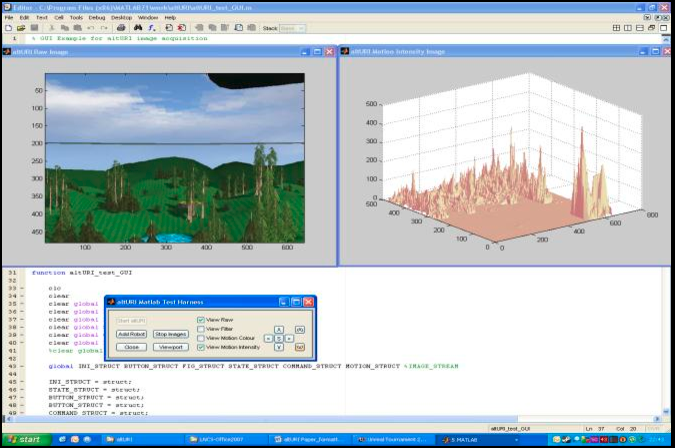
\includegraphics[width=0.45\textwidth]{chapter2/images/mdw_urbi.png}
    \caption{urbi middleware}
    \label{fig:mdw_urbi}
\end{figure}
เป็น open source สำหรับพัฒนาแอพพลิเคชั่นที่เกี่ยวข้องกับหุ่นยนต์หรือระบบที่มีความซับซ้อน ใช้ภาษาพื้นฐานเป็นภาษา C++ ติดต่อสื่อสารได้ภายในเครือข่ายเดียวกันเท่านั้น (Local Network)

\subsubsection*{MIRO}
\begin{figure}[!ht]
    \centering
    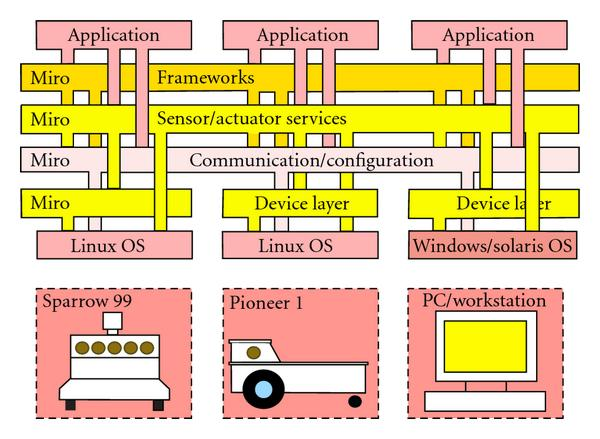
\includegraphics[width=0.45\textwidth]{chapter2/images/mdw_miro.jpeg}
    \caption{miro middleware}
    \label{fig:mdw_miro}
\end{figure}
เป็นกรอบการทำงานของหุ่นยนต์ที่เคลื่อนที่ได้โดยเขียนในลักษณะเป็น OOP

\subsubsection*{OpenRDK}
\begin{figure}[!ht]
    \centering
    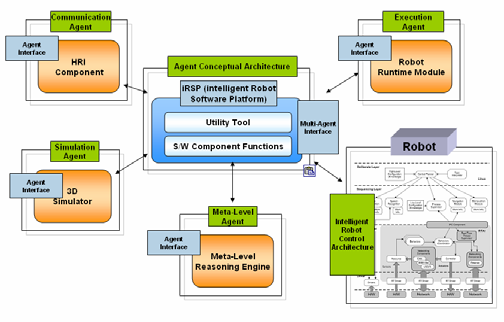
\includegraphics[width=0.45\textwidth]{chapter2/images/mdw_openrdk.png}
    \caption{openrdk middleware}
    \label{fig:mdw_openrdk}
\end{figure}
เป็น open source สำหรับพัฒนาระบบที่มีความเป็นอิสระต่อกัน (Modules) สามารถใช้ช่องทางการติดต่อสื่อสารและหน่วยความจำร่วมกันได้

\subsubsection*{Robot Operating System}
Robot Operating System หรือ ROS ถูกพัฒนาโดยบริษัท Willow Garage, แตเดิมแลว ROS ถูกพัฒนาเพื่อใช้
งานกับหุนยนต PR2 ในป 2007 ซึ่งพัฒนาเปน Open Source framework สําหรับนักพัฒนาซอฟแวรที่เกี่ยวของ
กับหุนยนต มีความสามารถในการทํางานแบบ parallel บนคอมพิวเตอรหลายๆเครื่องได สามารถทํางานไดหลาย
OS นอกจากนี้ยังมีคลังที่คอยเก็บซอฟแวรตางๆไวเปน libraries อีกดวย การใช ROS
จะชวยทําใหเราสามารถพัฒนาหุนยนตไดอยางรวดเร็วมากขึ้น ประหยัดเวลา ประหยัดทรัพยากร

\begin{figure}[!ht]
    \centering
    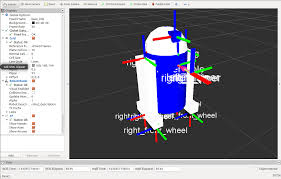
\includegraphics[width=0.5\textwidth]{chapter2/images/mdw_ros.jpeg}
    \caption{ROS middleware Rviz}
    \label{fig:mdw_ros}
\end{figure}
\begin{figure}[!ht]
    \centering
    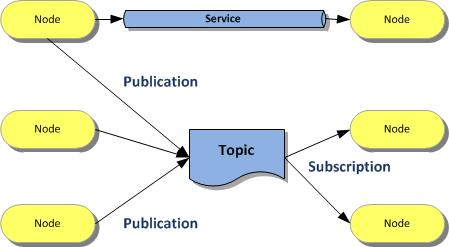
\includegraphics[width=0.5\textwidth]{chapter2/images/mdw_ros2.jpeg}
    \caption{ROS algitecture}
    \label{fig:mdw_ros2}
\end{figure}
\begin{figure}[!ht]
    \centering
    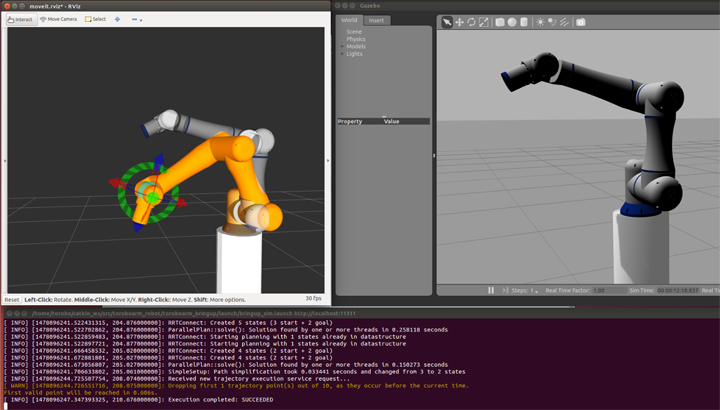
\includegraphics[width=0.5\textwidth]{chapter2/images/mdw_ros3.jpeg}
    \caption{ROS Moveit}
    \label{fig:mdw_ros3}
\end{figure}

\clearpage
\subsection{ระบบที่ใช้ในการจำลองการทำงานของหุ่นยนต์}
โปรแกรมจำลองการทำงานของหุ่นยนต์นั้นเป็นเครื่องมือที่สำคัญสำหรับนักวิจัยที่ทำงานวิจัยเกี่ยวกับหุ่นยนต์ การใช้โปรแกรมจำลองนั้นจะช่วยเพิ่มประสิทธิภาพในการทำงานหลายอย่าง
เช่น ให้รู้ว่าหุ่นยนต์ที่ออกแบบนั้นสามารถทำงานได้อย่างที่ต้องการหรือไม่ กระบวนการคิดถูกต้องหรือไม่
โปรแกรมจำลองระบบส่วนใหญ่จะคำนวณพลวัตของหุ่นยนต์โดยใช้เครื่องมือคำนวณ Open Dynamics Engine (ODE)

\subsubsection*{USARSim}
\begin{figure}[!ht]
	\centering
	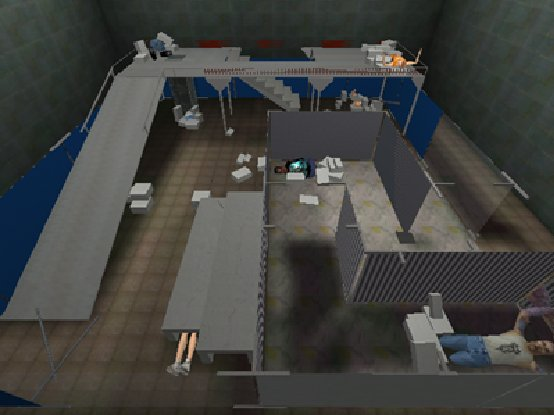
\includegraphics[width=0.5\textwidth]{chapter2/images/sim_USARSim.jpg}
    \caption{ผลลัพธ์จากการใช้โปรแกรม USARSim}
    \label{fig:sim_USARSim}
\end{figure}
USARSim เป็นโอเพนซอร์ซและเหมาะสำหรับทำหุ่นยนต์ประเภทกู้ภัยในซากเมือง โดยมีฐานการพัฒนามาจาก 
Unreal Tournament game engine ภายในโปรแกรมมีเครื่องมือสำหรับการทำงานวิจัย มีเซนเซอร์ของหุ่นยนต์ที่หลากหลาย 
เช่น เซนเซอร์รับภาพ หรือเซนเซอร์ตรวจความเคลื่อนไหว

\subsubsection*{MuRoSimF}
\begin{figure}[!ht]
    \centering
    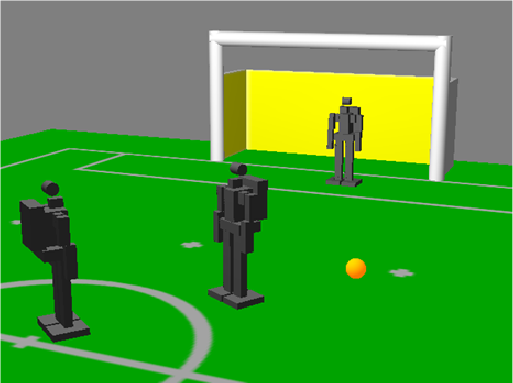
\includegraphics[width=0.5\textwidth]{chapter2/images/sim_MuRoSimF.png}
    \caption{ผลลัพธ์จากการใช้โปรแกรม MuRoSimF}
    \label{fig:sim_MuRoSimF}
\end{figure}
MuRoSimF ย่อมาจากคำว่า Multi-Robot Simulation Framework เป็นเครื่องมือที่ช่วยทำระบบจำลองจาก
Darmstadt University โปรแกรมระบบจำลองนี้มีการใช้งานที่ง่าย เหมาะสำหรับหุ่นยนต์หลายประเภท เช่น
หุ่นยนต์เคลื่อนที่ด้วยล้อ หุ่นยนต์สองขา หรือหุ่นยนต์หลายขา สามารถคำนวณพลวัตร และการกระทบกันของก้านต่อต่างๆได้

\clearpage
\subsubsection*{V-Rep}
\begin{figure}[!ht]
    \centering
    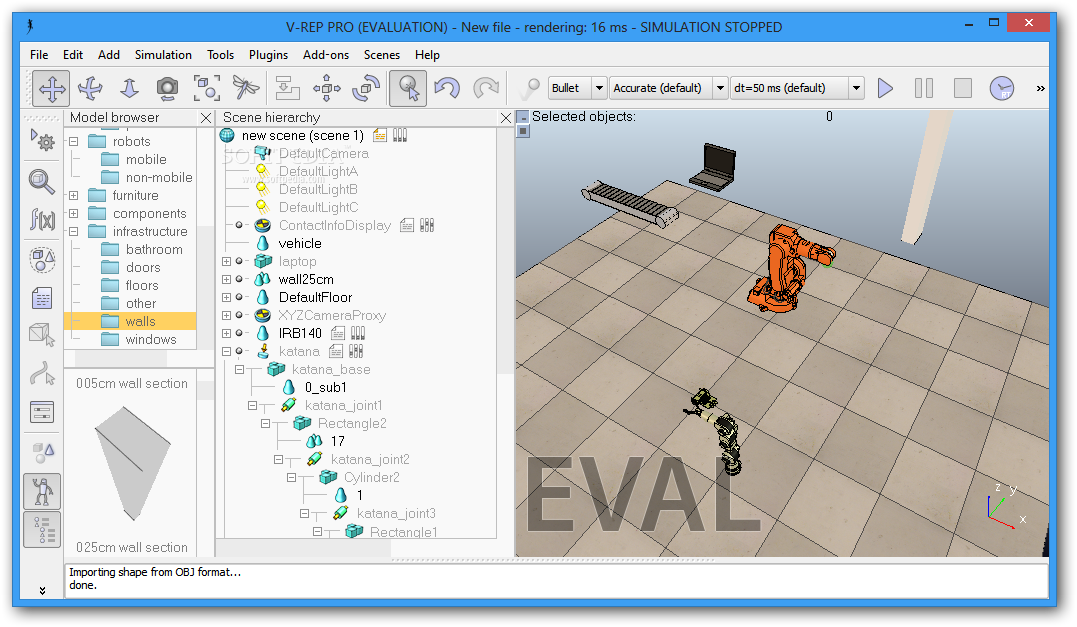
\includegraphics[width=0.7\textwidth]{chapter2/images/sim_vrep.png}
    \caption{ผลลัพธ์จากการใช้โปรแกรม V-REP}
    \label{fig:sim_vrep}
\end{figure}
VREP เป็นเครื่องมือสำหรับใช้ในการจำลองระบบหุ่นยนต์ ที่กำลังได้รับความนิยม โดยมีการเพิ่มระบบควบคุมผ่านโปรแกรมจากภายนอกเข้าไป สามารถที่จะเชื่อมต่อกับ ROS ได้และยังสามารถที่จะเขียน Script
เพื่อควบคุมหุ่นยนต์ผ่าน API ได้ 

VREP มีความเร็วในการประมวลผลที่สูง จำลองสายการผลิตในโรงงานอุตสหกรรม และเหมาะสำหรับหุ่นยนต์ที่มีการเคลื่อนที่ด้วยขา
มีเวอร์ชัน Education ที่เป็น Open source แต่หากจะใช้เพื่อการค้าจำเป็นจะต้องมี license เพื่อที่จะใช้งาน ราคาค่อนข้างสูง
\begin{figure}[!ht]
    \centering
    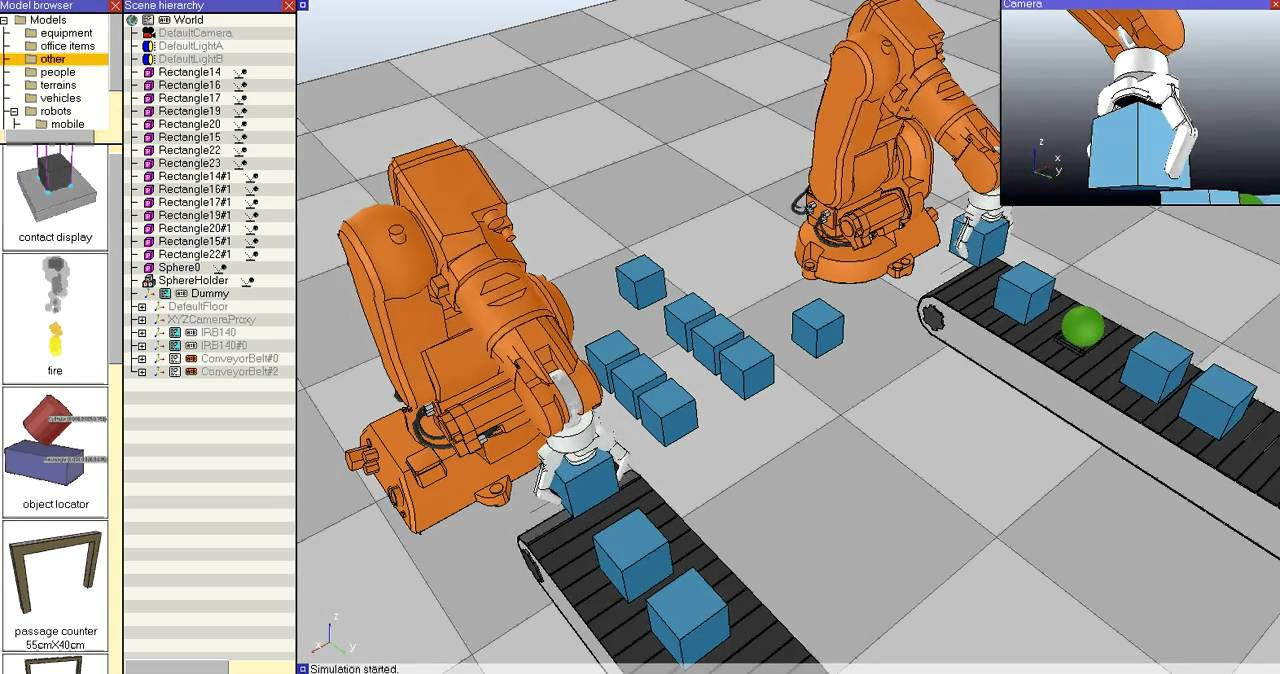
\includegraphics[width=0.7\textwidth]{chapter2/images/sim_vrep.jpg}
    \caption{V-REP จำลองสายการผลิต}
    \label{fig:sim_vrep2}
\end{figure}

\clearpage
\subsubsection*{Gazebo}
\begin{figure}[!ht]
    \centering
    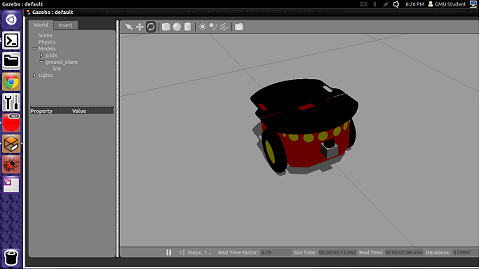
\includegraphics[width=0.5\textwidth]{chapter2/images/sim_gazebo1.png}
    \caption{Mobile robot with Gazebo}
    \label{fig:sim_gazebo1}
\end{figure}
\begin{figure}[!ht]
    \centering
    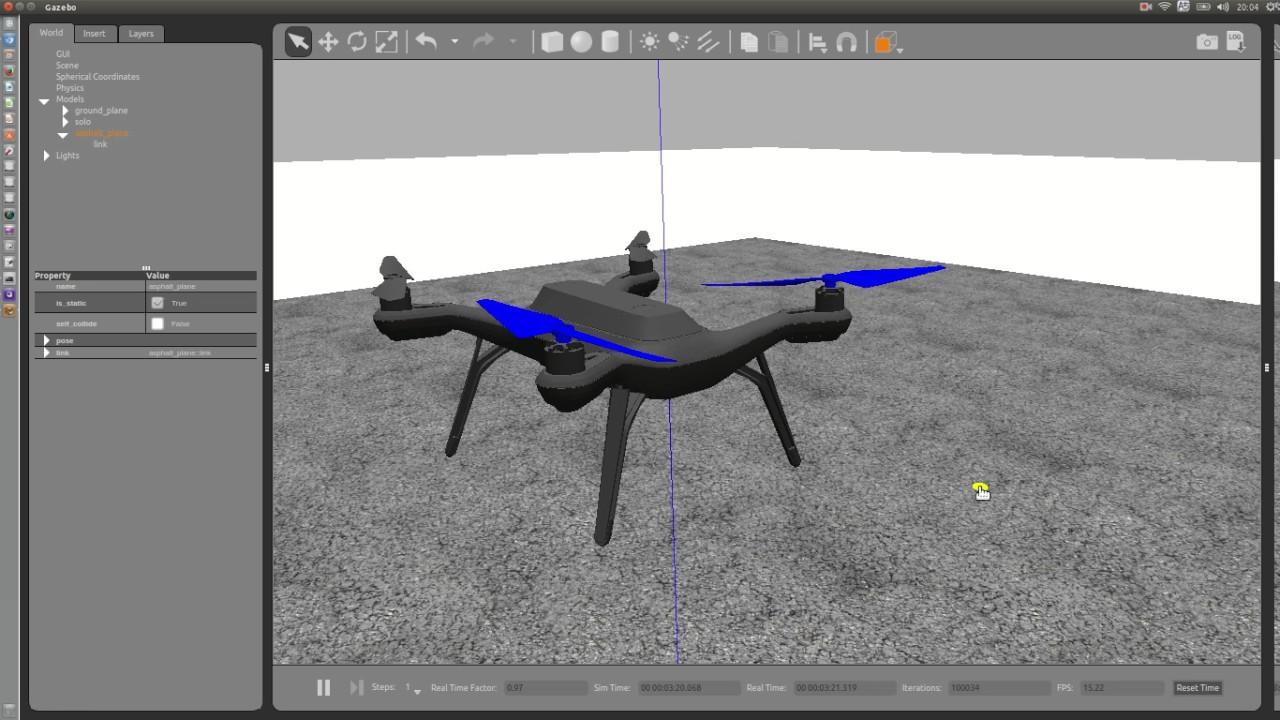
\includegraphics[width=0.5\textwidth]{chapter2/images/sim_gazebo2.jpg}
    \caption{Quadrotor with Gazebo}
    \label{fig:sim_gazebo2}
\end{figure}
Gazebo เป็นโปรแกรมจำลองการทำงานของหุ่นยนต์ ที่มีความสามารถในการคำนวณการเดินและการเคลื่อนที่ของหุ่นยนต์ที่สลับซับซ้อนได้
สามารถเห็นภาพกราฟฟิคของหุ่นยนต์ขณะทำงาน โดยผู้ใช้สามารถกำหนดค่าตัวแปรทางฟิสิกส์ต่าง ๆได้ เช่นน้ำหนัก ค่าความเฉื่อย แรงเสียดทานของข้อต่อ
ทำให้การออกแบบหุ่นยนต์หรือทดลองโปรแกรมได้เหมือนกับโลกจริง มีแสง มีเงา และ พื้นผิวของวัตถุ และที่พิเศษคือสามารถสังเคราะห์ค่าของเซนเซอร์
เซนเซอร์พร้อมสัญญาณรบกวน ค่าระยะทาง แรงบิด และอื่นๆ คำนวณพลศาสตร์ของหุ่นยนต์โดยใช้ตัวคำนวณทางฟิสิกส์เป็น Bullet หรือ Simbody
ในการจำลองหุ่นยนต์ในโปรแกรมนี้จำเป็นต้องได้รับไฟล์ข้อมูลของหุ่นยนต์มาก่อนซึ่งอยู่ในรูปแบบของ URDF ซึ่ง URDF คือ
ประเภทของไฟล์ที่บ่งบอกถึงความสัมพันธ์ของข้อต่อและก้านต่อแต่ละชิ้นในตัวหุ่นยนต์ มีความสามารถในการอธิบายถึงกลศาสตร์และการเคลื่อนที่ของหุ่นยนต์
รวมถึงตรวจสอบการกระทบกันของก้านต่อในหุ่นยนต์ได้ ภายในไฟล์นี้จะประกอบไปด้วย

\paragraph*{Link :}
คือก้านต่อของหุ่นยนต์ซึ่งภายในจะสามารถบอกขนาด รูปร่าง สี และสามารถ import 3d mesh เข้ามาได้ด้วย
อีกทั้งยังสามารถใส่รายละเอียดของการเคลื่อนที่ของก้านต่อได้เช่น inertial matrix และ collision properties

\paragraph*{Joint :}
คือข้อต่อของหุ่นยนต์สามารถกำหนดกลศาสตร์และการเคลื่อนที่ได้เช่น Joint limits ของข้อต่อที่กำลังหมุนและความเร็วการหมุน
ซึ่งข้อต่อมีหลายแบบที่สามารถกำหนดได้เช่น ข้อต่อแบบหมุน, ข้อต่อแบบเลื่อน, ข้อต้อต่อแบบยึดติด, ข้อต่อแบบต่อเนื่อง

%%%%%%%%%%%%%%%%%%%%%%%%%%%%%%%%%%%%%%%%%%%%%%%%%%%%%%%%%%%%%%%%%%%%
\clearpage
\subsection{Robot Operating System}
Robot Operating System หรือ ROS ถูกพัฒนาโดยบริษัท Willow Garage, แต่เดิมแล้วเค้าพัฒนาเพื่อใช้งานกับหุ่นยนต์ PR2 ในปี 2007
ซึ่งพัฒนาเป็น open source framework สำหรับนักพัฒนาซอฟแวร์ที่เกี่ยวข้องกับหุ่นยนต์ มีความสามารถในการทำงานแบบ parallel
บนคอมพิวเตอร์หลายๆเครื่องได้ สามารถทำงานได้หลาย OS แต่ที่ซัพพอร์ทจริงๆคือ Ubuntu และ Debian นอกจากนี้ยังมีคลังที่คอยเก็บซอฟแวร์ต่างๆไว้เป็น
libraries อีกด้วย การใช้ ROS จะช่วยทำให้เราสามารถพัฒนาหุ่นยนต์ได้อย่างรวดเร็วมากขึ้น ประหยัดเวลา ประหยัดทรัพยากร
ในส่วนนี้จะกล่าวถึง ROS คร่าวๆ

\subsubsection*{Node}
Node เป็นเหมือนหน่วยประมวลผลในระบบ ROS, Node สามารถที่จะส่งข้อมูลหา Node อื่นๆได้ ผ่าน Topics หรือ Services
ในทางปฏิบัติแล้ว Node เป็นตัวประมวลผลย่อยๆ ที่คอยทำหน้าที่เฉพาะ ยกตัวอย่างเช่น Node ตัวแรกเชื่อมต่อกับกล้อง
เพื่อที่จะนำภาพจากกล้องออกมา  Node ตัวที่สองใช้ในการหาลูกบอลที่อยู่ในภาพที่ได้มาจาก Node ตัวแรก และ Node ตัวที่สามใช้ในการคำนวณหาตำแหน่งของลูกบอลที่อยู่บนโลกจริงๆ
จากตำแหน่งของลูกบอลที่ได้มาจาก Node ที่สอง ดังนั้นจะเห็นว่าแต่ละ Node จะทำงานเฉพาะของตัวเอง ซึ่งสามารถนำมารวมกันได้ การเขียนเป็นแบบ Node จะช่วยทำให้เราสามารถที่จะนำโปรแกรมกลับมา
แก้ไขปรับปรุงให้ใช้ใหม่ได้ง่าย ในกรณีที่จะนำไปทำงานอย่างอื่น ยกตัวอย่างเช่น  Node ที่เอาภาพจากกล้องออกมา อาจจะมี Node อีกตัว ทำหน้าที่ในการหาโกลด์เป้าหมาย และหาทิศทางการเคลื่อนที่ของหุ่นยนต์ได้
ดังนั้นการพัฒนา Node เป็นส่วนย่อยๆเล็กๆ ก็เพื่อที่จะทำให้การแก้ไขหรือปรับปรุงได้ง่าย
\begin{figure}[!ht]
	\centering	    
	\begin{tikzpicture}[shorten > = 1pt,scale=0.9, transform shape]
		% Place nodes
		\node [node] (image_provider) {image\_provider};
		\node [topic, below of=image_provider] (/image) {/image\\sensor\_msgs/Image.msg};
		\node [node, below left of=/image] (line_detection) {line\_detection};
		\node [node, below right of=/image] (stop_detection) {stop\_detection};
		\node [topic, below of=line_detection,xshift=-0.5cm] (/line) {/line\\example\_msgs/Line.msg};
		\node [topic, below of=stop_detection,xshift=0.5cm] (/stop) {/stop\\example\_msgs/Stop.msg};
		\node [node, below of=/image, yshift=-3.0cm] (navigation) {navigation};
		\node [topic, below of=navigation] (/cmd_vel) {/cmd\_vel\\geometry\_msgs/Twist.msg};
		\node [node, below of=/cmd_vel,yshift=1cm] (robot_control) {robot\_control};
		% % Draw edges
		\path [line] (image_provider) -- (/image);
		\path [line] (/image) -- (line_detection);
		\path [line] (/image) -- (stop_detection);
		\path [line] (line_detection) -- (/line);
		\path [line] (stop_detection) -- (/stop);
		\path [line] (/line) -- (navigation);
		\path [line] (/stop) -- (navigation);
		\path [line] (navigation) -- (/cmd_vel);
		\path [line] (/cmd_vel) -- (robot_control);
	\end{tikzpicture}
	\caption{ตัวอย่างสถาปัตยกรรมของ ROS}
	\label{fig:ros_architecture}
\end{figure}

จากตัวอย่างสถาปัตยกรรมของ ROS ดังรูปที่ \ref{fig:ros_architecture} นั้นสามารถอธิบายได้ว่า หุ่นยนต์เคลื่อนที่ด้วยล้อมีภารกิจคือ
เคลื่อนที่ตามเส้นไปเรื่อยๆจนกว่าจะเจอเครื่องหมายหยุด Node คือตัวที่แสดงด้วยรูปวงรี ข้างในเป็นชื่อ Node  ส่วน Topic จะแสดงด้วยรูปสี่เหลี่ยม
ซึ่งข้างในเป็นชื่อของ Topic และชนิดของ Message ที่ใช้ในการส่งข้อมูล, มาดูกันก่อนอื่น ภาพถูกส่งมาจากกล้อง และก็มี Node สองตัวในการดูเส้น และเครื่องหมายหยุด
จากภาพที่ได้มา เมื่อ Node ได้ข้อมูลแล้วก็นำมาประมวลผลการเดินของหุ่นยนต์โดยส่งไปยัง node navigation และ Node นี้ก็จะทำหน้าที่คำนวณความเร็วและทิศทางของหุ่นยนต์
ส่งไปยัง node robot\_control ซึ่งเป็นตัวสั่งการมอเตอร์ของหุ่นยนต์อีกทีหนึ่ง
\begin{table}[!ht]
	\begin{subtable}[h]{0.40\textwidth}
		\centering
		\begin{tabular}{| p{4cm}| p{1.5cm} |}
			\hline 
			\multicolumn{2}{|c|}{Twist.msg} \\
			\hline
			geometry\_msgs/Vector3 & linear  \\
			geometry\_msgs/Vector3 & angular \\
			\hline  
		\end{tabular}
		\caption{Message Twist}
		\label{tab:message_twist}
	\end{subtable}
	\hfill
	\begin{subtable}[h]{0.40\textwidth}
		\centering
		\begin{tabular}{| p{1.5cm}| p{2.5cm} |}
			\hline 
			\multicolumn{2}{|c|}{Stop.msg} \\
			\hline
			uint8   & RED = 0   \\
			uint8   & GREEN = 1 \\
			uint8   & color     \\
			float32 & distance  \\
			\hline  
		\end{tabular}
		\caption{Message Stop}
		\label{tab:message_stop}
	\end{subtable}
	\caption{ตัวอย่างชื่อและข้อมูลของ Message}
	\label{tab:message_example}
\end{table}

ตัวอย่างของ Message สองอันนี้ Twist message ดังรูปที่ \ref{tab:message_twist} คือ message ที่เอาไว้บอกความเร็วเชิงเส้น และความเร็วเชิงมุม
ซึ่ง ROS มี message ชนิดนี้ให้อยู่แล้ว ส่วน Stop message ดังรูปที่ \ref{tab:message_stop} คือ message ที่เอาไว้บอกระยะทางและสีของป้าย Stop
ซึ่ง message นี้ถูกสร้างขึ้นมาใหม่เพื่อใช้กับงานนี้โดยเฉพาะ

\subsubsection*{Topics and Messages}
Messages เป็นตัวหลักสำคัญในการติดต่อสื่อสารกันระหว่าง Node ใน ROS โดยที่ message จะถูกส่งผ่านไปยัง topic เสมอ
แต่ละ Node สามารถที่จะ subscribe หรือ publish ไปกี่ topic ก็ได้ การเชื่อมต่อกันระหว่าง Node นั้นสามารถส่งอยู่ภายในเครื่องคอมพิวเตอร์เครื่องเดียวกัน
หรือเครื่องอื่นได้ที่อยู่ใน network เดียวกัน โดยจะติดต่อสื่อสารโดยใช้ TCP/IP การใช้คอมพิวเตอร์หลายเครื่องก็จะช่วยให้การประมวลผลมีประสิทธิภาพมากยิ่งขึ้น
นอกจากนั้นยังสามารถที่จะแบ่งหน้าที่การทำงานออกจากกันได้ เราสามารถที่จะสร้าง Topic หรือ Message ขึ้นมาเองได้
หากต้องการใช้งานที่เฉพาะทาง

\subsubsection*{roscore}
roscore เป็นส่วนกลางในการรันระบบทั้งหมด เราจะเรียกกันว่า rosmaster ซึ่งมีหน้าที่ในการจัดการ
topics ทั้งหมด ที่ต้องการจะเชื่อมต่อกันไม่ว่าจะเป็นการ publish หรือ subscribe แต่ rosmaster
จะเป็นแค่ตัวจัดการเท่านั้นไม่ได้เป็นตัวที่เก็บ message ต่างๆที่ส่งไปมา ดังนั้น rosmaster จะไม่ทำให้เกิดคอขวด เวลารันระบบ
ในกระบวนการก็คือ subscribe node จะถาม rosmaster ว่ามี topic ที่ตัวเองต้องการรับข้อมูลไหม
ส่วนตัว master ที่เก็บค่า topic message เอาไว้ ก็จะส่งไปยัง subscribe node ถ้าหากมีชื่อตรงตามที่ร้องขอมา
และ rosmaster ก็จะจำไว้ว่ามี node ไหนเชื่อมต่อกับ node ไหนบ้าง

rosparameter server เป็นตัวในการเก็บค่าต่างๆที่เป็น global key-value ซึ่งช่วยให้ node ทุกตัวสามารถใช้ข้อมูลตัวเดียวกันได้
สามารถปรับเปลี่ยนระหว่างการทำงานอยู่ได้ โดยใช้ rqt plugin ซึ่งจะกล่าวในส่วนถัดไป

roslog เป็นตัวที่ใช้สำหรับ logging ข้อมูลต่างๆ ซึ่งจะถูก publish ออกมาทาง topic /rosout ซึ่งเราสามารถที่จะเขียนโปรแกรม
subscribe จากตัว topic นี้ไปเก็บเป็นไฟล์ได้

%%%%%%%%%%%%%%%%%%%%%%%%%%%%%%%%%%%%%%%%%%%%%%%%%%%%%%%
\subsubsection*{Services}
Services หรืออีกชื่อหนึ่งคือ remote procedure calls (RPC) เป็นการส่ง messages แบบที่ไม่ได้เจาะจงว่าจะส่งไปที่ไหน
เมื่อ service ถูกเรียกแล้วระบบจะรอจนกว่าจะมีการตอบกลับ เราจะเรียกกระบวนการนี้ว่า request และ response message
Node ที่คอยทำงานเมื่อมีการเรียกใช้ service จะเรียกว่า service server และ node ที่เรียก service จะเรียกว่า service client
การใช้งาน service เหมาะสำหรับงานที่ต้องการความรวดเร็ว (fast task) แต่ไม่ควรใช้กับระบบที่ต้องใช้เวลานาน
เพราะระบบจะหยุดไม่ยอมทำต่อ ต้องรอให้ service ทำงานเสร็จก่อน สำหรับงานที่ต้องใช้เวลาในการคำนวณนานจะไปใช้ action
แทน จะกล่าวในส่วนถัดไป 

\subsubsection*{Actions}
Actions จะใช้กับการทำงาน การประมวลผลที่ต้องใช้เวลานานในการทำงาน หรือที่เรียกว่า asynchronously task
ในแต่ละ action จะมี message อยู่ 3 ชนิด คือ goal, feedback และ result Node ที่เป็นตัวรันและรอให้ node อื่นมากเรียก
จะเรียกว่า action server ส่วน node ที่เรียกการทำงาน action จะเรียกว่า action client การใช้งาน action จะเริ่มจาก
action client จะส่ง message goal ไปยัง action server แล้ว action server จะพยายามทำตาม goal ที่ได้รับมา ในระหว่างที่
action client ก็จะทำงานของตัวเองต่อไป แต่จะได้รับ feedback จาก action server อยู่ตลอดเวลา และเมื่อถึง goal ที่กำหนดแล้ว
server จะแจ้งมาทาง result message

\subsubsection*{Code Organization}
ส่วนที่เล็กที่สุดของการจัดการซอฟแวร์ใน ROS ก็คือ package ภายใน package จะมีไฟล์ที่ชื่อว่า package.xml
ซึ่งไฟล์นี้จะทำหน้าที่ในการ อธิบายและบอกข้อมูลต่างๆที่เกี่ยวกับ package นี้ ยกตัวอย่างเช่น
ชื่อของ package, ชื่อของผู้เขียน, ลิขสิทธ์ และ dependencies ที่ต้องใช้กับ package นี้
นอกจากนี้ยังสามารถใส่ข้อมูลอื่นๆเกี่ยวกับ node ลงไปเพิ่มเติมได้

\begin{figure}[!ht]
	\begin{Verbatim}[fontsize=\small]
<package>
	<name>example_package</name>
	<version>1.0.0</version>
	<description>Short example for a package.xml.</description>
	<maintainer emanil="ex@example.org">Jane Doe</maintainer>
	<license>BSD</license>
	<buildtool_depend>catkin</buildtool_depend>
	<build_depend>example_2</build_depend>
	<run_depend>std_msgs</run_depend>
</package>
	\end{Verbatim}
	\caption{ตัวอย่างไฟล์ package.xml}
    \label{fig:example_packagexml}
\end{figure}

แต่ละ tags ใช้ในการบอกข้อมูลของ package นี้ ใครเป็นเจ้าของ ใครเป็นคนเขียน รวมไปถึง dependencies
ที่จำเป็นต้องใช้ของ package นี้ด้วย ดังรูปที่ \ref{fig:example_packagexml} 

%%%%%%%%%%%%%%%%%%%%%%%%%%%%%%%%%%%%%%%%%%%%%%%%%%%%%%%
\clearpage
\subsubsection*{Code Distribution}
การที่จะนำ Nodes กลับมาใช้ใหม่หรือเอาออกมาแบ่งปันให้ผู้อื่นได้นั้น จะต้องมีการทำเอกสารของ Packages นั้นๆด้วย
โดยปกติแล้วจะถูกนำไปเก็บไว้ที่ GitHub และ package dependencies จะบอกไว้ในไฟล์ package.xml
เรียบร้อยแล้ว เพื่อให้ง่ายต่อการนำไปติดตั้ง หากผู้ที่นำไปใช้พัฒนาต่อหรือแก้ไขข้อผิดพลาดก็สามารถที่จะช่วยกันได้
โดยการ Pull request หรือ Report issues ได้

%%%%%%%%%%%%%%%%%%%%%%%%%%%%%%%%%%%%%%%%%%%%%%%%%%%%%%%
\subsubsection*{ROS Packages ที่ใช้ในงานวิจัย}
Package คือพื้นฐานของ ROS, แอพพลิเคชั่นทั้งหมดใน ROS จะพัฒนาโดยมี package เป็นรากฐาน ใน package นั้นจะเก็บพวกไฟล์
configuration ไปจนถึงไฟล์ launch ที่สามารถไปรัน package หรือ node อื่นๆได้ ตอนนี้ ROS มี packages มากกว่า 5000 packages แล้ว

Metapackage เป็นการรวมกันของ packages ที่ทำหน้าที่คล้ายๆกันหลายๆตัวมารวมไว้ที่เดียวเพื่อจะได้ใช้งานง่าย
ตัวอย่าง Navigation metapackage ประกอบไปด้วย 10 packages เช่น [AMCL (partical filter), DWA, EKF (extended kalman filter) 
และ map\_server] ซึ่งหากติดตั้ง metapackage ตัวนี้ก็จะได้มาหมดเลย

ในส่วนนี้จะอธิบายคร่าวๆถึง ROS standard packages ที่จะเอามาใช้ในงานวิจัยครั้งนี้

\paragraph*{rosbag}
rosbag เป็นแพกเกจที่สามารถบันทึก message ที่ส่งหากันในระหว่างที่ ROS กำลังทำงานได้
ไฟล์ที่บันทึกจะเรียกว่า rosbag ประโยชน์ของมันคือเราสามารถเอาเข้ามาใช้ในการตรวจสอบ
หรือนำมาเล่นซ้ำได้ อีกทั้งยังง่ายต่อการค้นหาข้อผิดพลาดอีกด้วย

\paragraph*{tf2}
tf2 เป็นแพกเกจที่สามารถติดตามการเปลี่ยนแปลงของ Coordinate frame เราสามารถใช้ในการหาความสัมพันธ์ระหว่าง
frame ได้ ยกตัวอย่างเช่นหากเราต้องการหาตำแหน่งของ foot เทียบกับ pelvis ก็สามารถใช้ tf2 หาได้

\paragraph*{robot\_state\_publisher}
robot\_state\_publisher แพกเกจที่ subscribe JointState message เพื่อที่จะนำตำแหน่งของของข้อต่อ
และแปลงให้อยู่ในรูปข้อมูลของ tf2, tf2 สามารถเรียกจาก Node ใดๆก็ได้เพื่อที่จะหา Coordinate frame ที่ต้องการได้

\paragraph*{URDF}
Unified Robot Description Format (URDF) เป็นไฟล์ XML ที่เอาไว้อธิบายลักษณะของหุ่นยนต์
ใน ROS มีแพกเกจที่ใช้สำหรับการอ่านไฟล์ คือ urdf\_parser แต่ไฟล์นี้ก็มีการใช้งานโดย tf2 เช่นกัน

\paragraph*{xacro}
xacro เป็นไฟล์ XML เช่นเดียวกับ URDF โดยไฟล์ xacro นี้มีประโยชน์มากในการใช้งานใน ROS เพราะว่าทำให้การเขียนไฟล์
URDF ง่ายขึ้น เพราะสามารถทำเป็นมาโครได้ สามารถปรับแต่งค่าตัวแปรต่างๆได้ง่ายขึ้น

%%%%%%%%%%%%%%%%%%%%%%%%%%%%%%%%%%%%%%%%%%%%%%%%%%%%%%%
\clearpage
\subsubsection*{การแสดงผลด้วยภาพ}
จุดแข็งสำคัญของ ROS อีกอย่างคือ มีเครื่องมือที่ช่วยในการแสดงผลด้วยภาพได้ที่นอกเหนือจากระบบ
publisher-subscriber การใช้เครื่องมือการแสดงผลด้วยภาพนี้จะช่วยให้การทำงานง่ายขึ้นและประหยัดเวลามากขึ้น
ในการนำข้อมูลต่างๆจากหุ่นยนต์ออกมาแสดงผล เพราะว่าเครื่องมือแสดงผลภาพนี้สามารถที่จะ subscribe
จาก topic ที่มีการใช้งานอยู่แล้วมาแสดงผลได้ทันที ใน ROS มีเครื่องมือสำคัญอยู่ 2 ตัวที่ใช้สำหรับการแสดงผลด้วยภาพ
ซึ่งสามารถที่จะปรับแต่งให้กลายเป็นเวอร์ชั่นของเราเองได้

\paragraph*{rqt}
rqt เป็น UI ที่มีฐานมาจาก QT ซึ่งมาพร้อมกับการเชื่อมต่อ ROS เป็นส่วนเสริมในรูปแบบของ QtWidget
เราสามารถที่จะแสดงผลหลายๆ widgets ได้ภายในเวลาเดียวกัน สามารถที่จะย่อขยาย เปลี่ยนตำแหน่ง
ลากวางได้ การเชื่อมต่อกับ ROS นั้นสามารถนำการแสดงผลภาพแบบ 2D ไปแสดงได้ดังรูปที่ \ref{fig:ros_gui_example}
เป็นการแสดงภาพของกราฟที่ได้รับข้อมูลมาจาก topic หลายๆตัว และสามารถที่จะปรับแต่งค่าและ publish
ออกไปได้ด้วยการเขียนโปรแกรมเข้าไป ซึ่งจะเป็นประโยชน์อย่างมากเวลาที่ใช้ในการปรับจูนพารามิเตอร์ต่างๆ
เพราะว่าเราสามารถที่จะเปลี่ยนค่าได้ทันที ไม่ต้องรันโปรแกรมใหม่ ในรูปที่ \ref{fig:ros_gui_example}
เป็นการนำ rqt มาเขียนเป็น GUI ให้ผู้ใช้สามารถใช้งานได้ง่ายและสามารถที่จะปรับแต่งพารามิเตอร์ต่างๆได้เรียลไทม์

\begin{figure}[!ht]
    \centering
    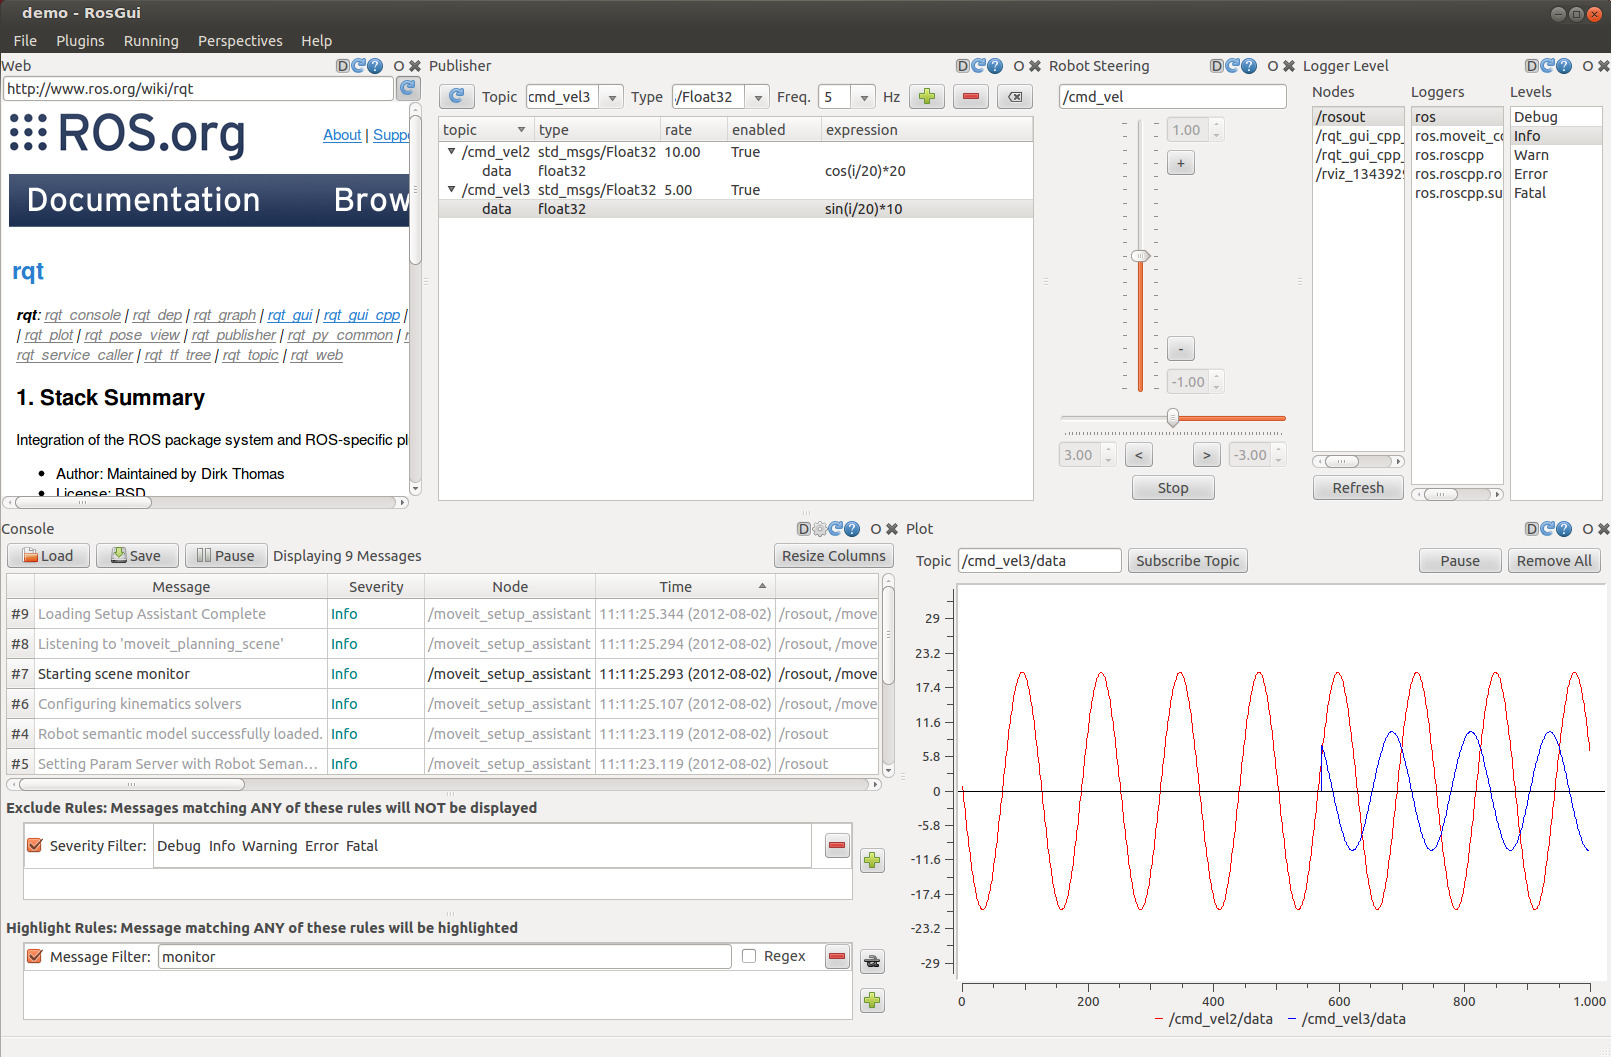
\includegraphics[width=0.8\textwidth]{chapter2/images/ros_gui_example.png}
	\caption{ตัวอย่างการแสดงผลใน rqt }
    \label{fig:ros_gui_example}
\end{figure}

\paragraph*{RViz}
RViz เป็นการแสดงผลด้วยภาพแบบสามมิติของสถานะต่างๆของหุ่นยนต์และสภาพแวดล้อม โดยใช้ไฟล์ URDF เป็นมาตรฐานการแสดงถึงหุ่นยนต์
ซึ่งสามารถที่จะแสดงตำแหน่งปัจจุบันของข้อต่อต่างๆในหุ่นยนต์ได้ สามารถที่จะแสดงค่าเซนเซอร์เป็น marker ได้
การใช้งานจะเป็นเหมือนการบอกพิกัดเฟรม ลักษณะการแสดงผลใน RViz มีหลากหลายรูปแบบไม่ว่าจะเป็น
camera images, depth clouds, laser scans หรือ point clouds อย่างไรก็ตามการแสดงผลใน Rviz
นั้นจะไม่ได้คำนึงถึงแรงที่เข้ามากระทำกับตัวของหุ่นยนต์ แต่ถ้าเป็นการเคลื่อนที่ ที่มีพิกัดเฟรมแล้วสามารถเอามาแสดงได้
ดังรูปที่ \ref{fig:example_visualization_rviz} เป็นตัวอย่างของหุ่นยนต์เคลื่อนที่ด้วยล้อ และทำแผนที่ด้วยข้อมูลความลึกที่ได้มาจาก Kinect

\clearpage
\begin{figure}[!ht]
    \centering
    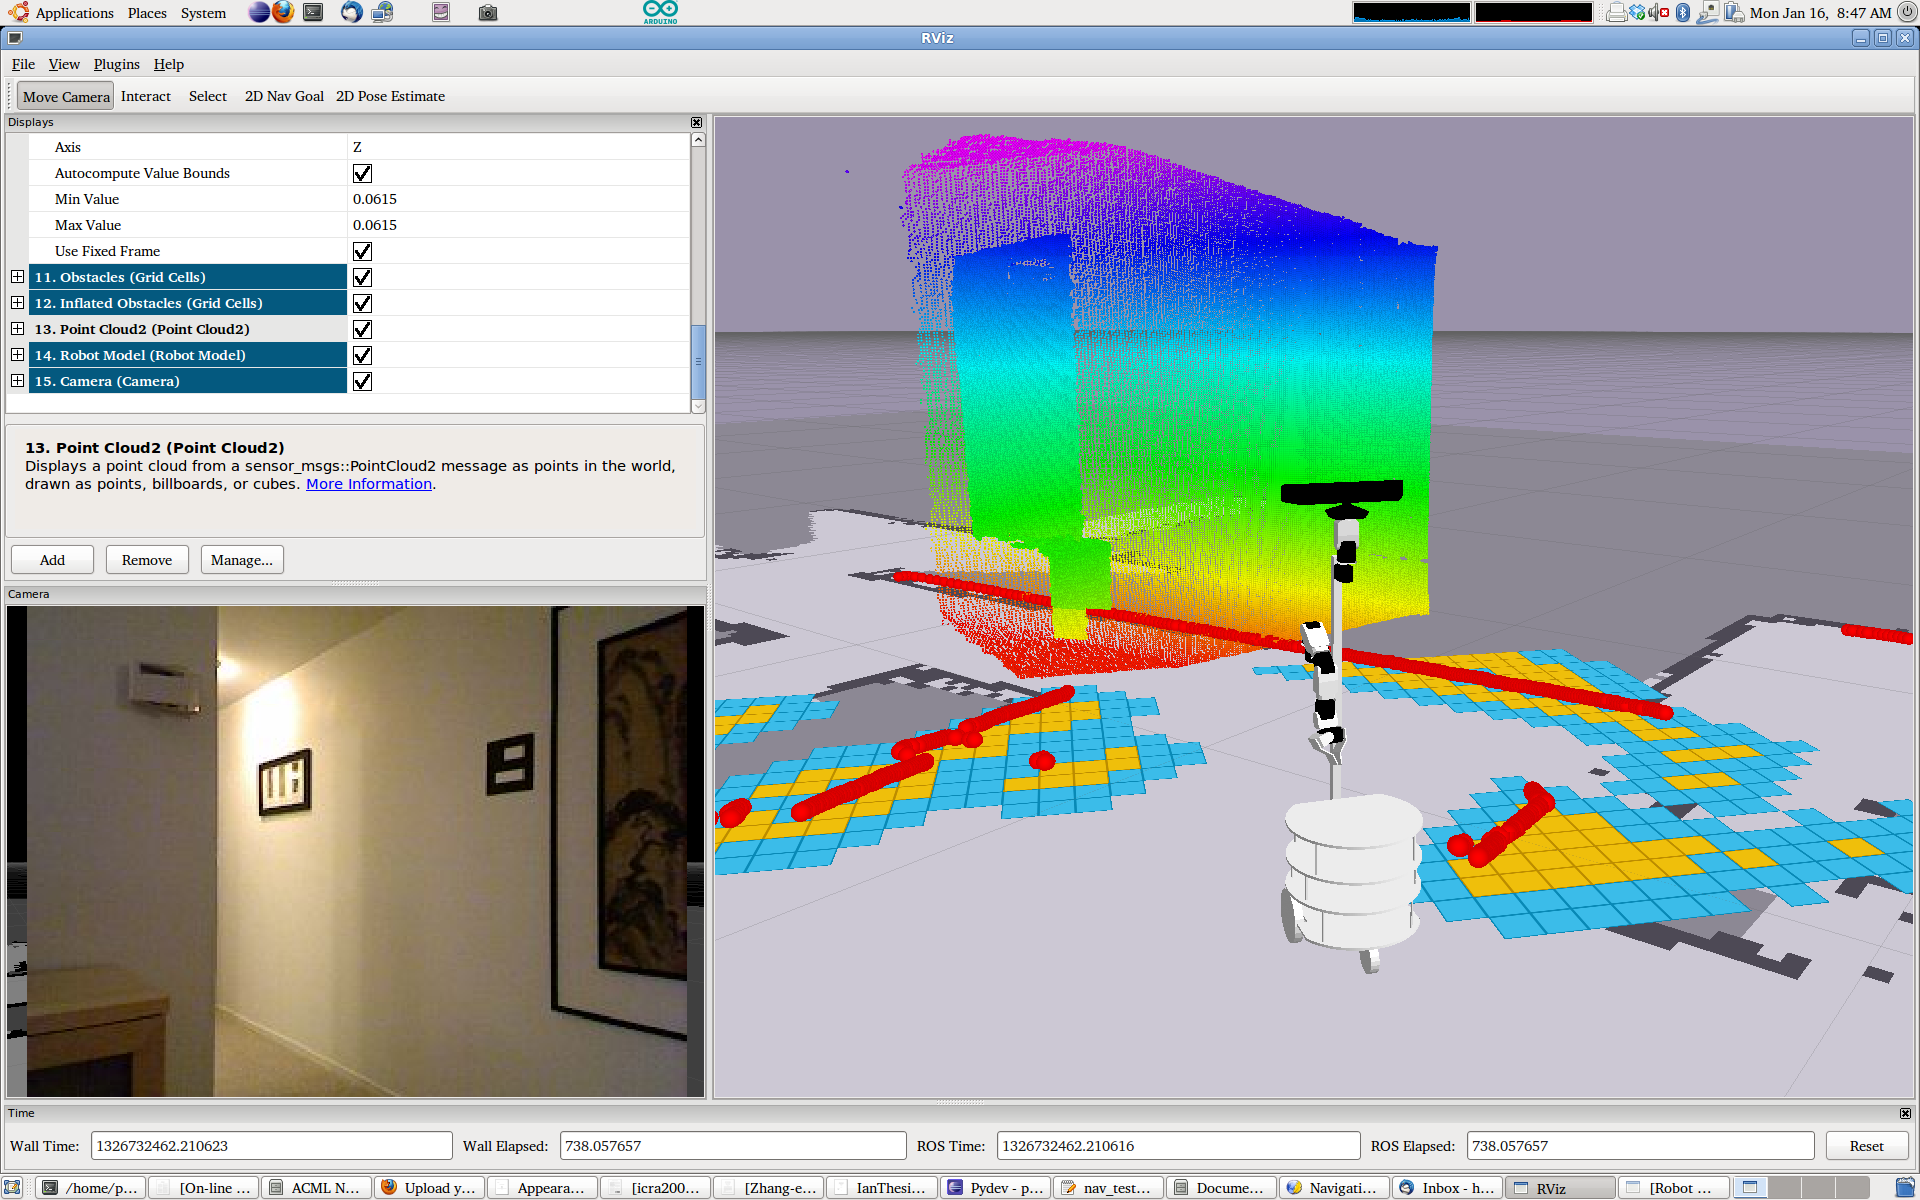
\includegraphics[width=0.8\textwidth]{chapter2/images/nav_test_rviz_2.png}
	\caption{ตัวอย่างการแสดงผลใน RViz}
    \label{fig:example_visualization_rviz}
\end{figure}

\subsubsection*{ระบบจำลอง}
ระบบจำลองเป็นส่วนที่สำคัญมากสำหรับการพัฒนาโปรแกรมของหุ่นยนต์ เพราะว่าเราสามารถที่จะสร้างโปรแกรมและ
ทดสอบได้โดยไม่จำเป็นต้องมีฮาร์ดแวร์ ซึ่งในส่วนนี้จะช่วยลดความเสียหายจากบักหรือโปรแกรมที่ผิดพลาด ที่อาจจะเกิดขึ้นกับหุ่นยนต์ได้
การจำลองจะช่วยลดเวลาในการพัฒนาลงได้ ระบบจำลองปัจจุบันมีมากมายหลายตัวแต่ ตัวที่ได้รับคำแนะนำมากที่สุดคือ Gazebo
เพราะว่า Gazebo สามารถที่จะเชื่อมต่อกับ ROS ได้โดยตรง และนักพัฒนาส่วนใหญ่ใช้ Gazebo

การจะใช้ Gazebo ได้นั้นเราจะต้องใช้ไฟล์ URDF ซึ่งเป็นไฟล์ที่เอาไว้แสดงหุ่นยนต์ในระบบจำลอง และสามารถที่จะคำนวณหา collision
ให้เราได้อีกด้วย

\begin{figure}[!ht]
    \centering
    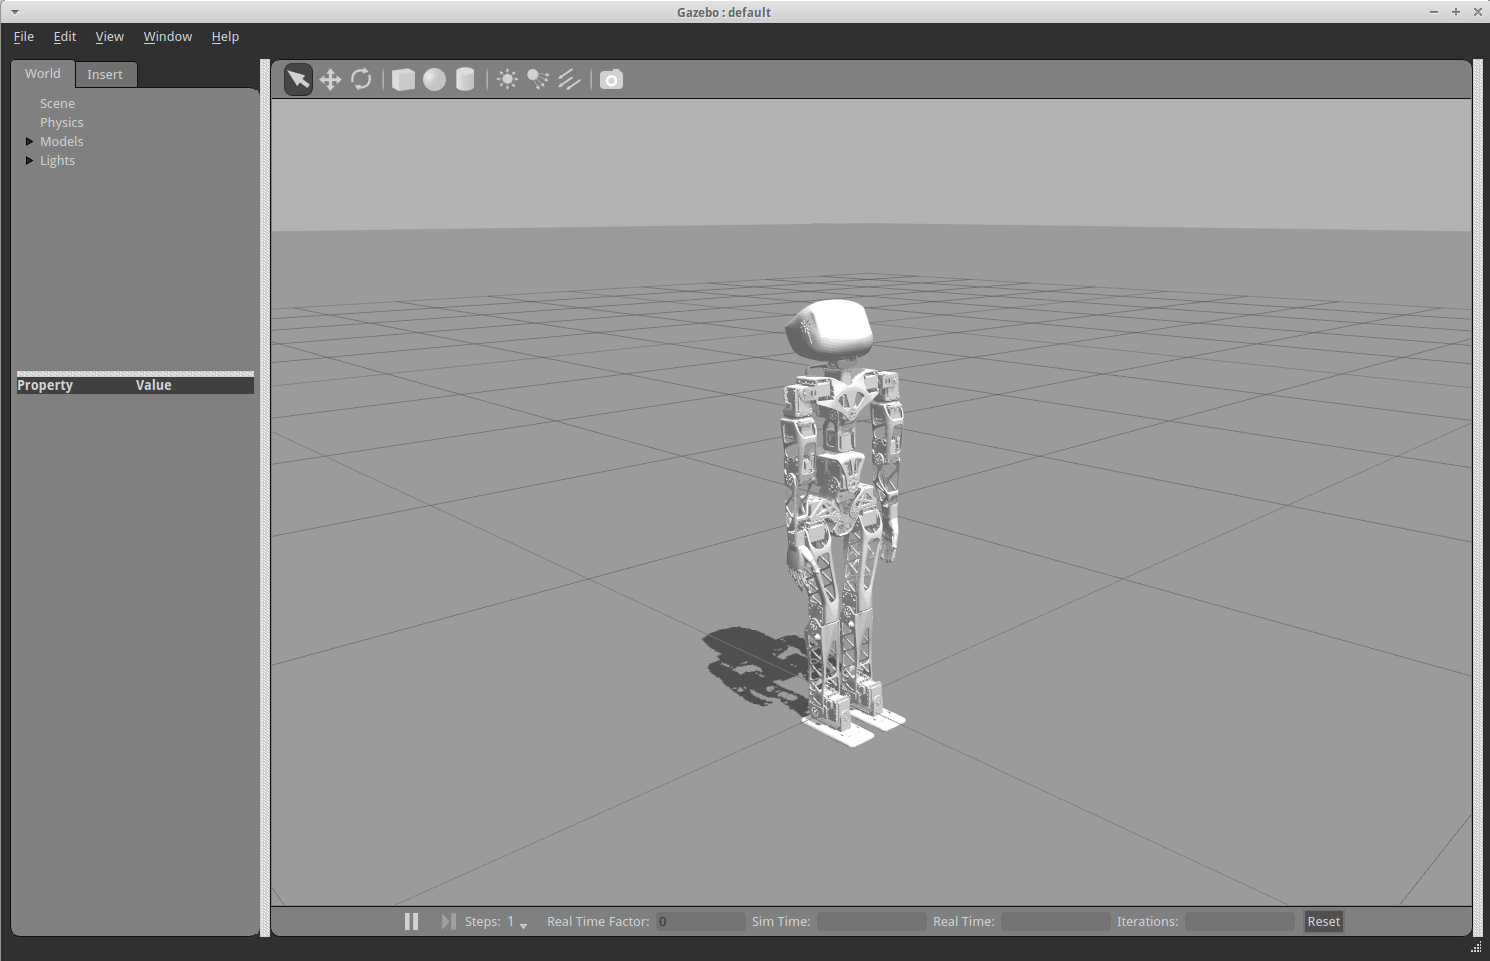
\includegraphics[width=0.8\textwidth]{chapter2/images/gazebo_poppy.png}
	\caption{ตัวอย่างหุ่นยนต์ฮิวมานอยด์ Poppy}
    \label{fig:gazebo_poppy}
\end{figure}

